\documentclass[12pt,a4paper,twoside]{ipb}

% comentar caso seja uma disseração de mestrado
% \usepackage{projei}

\usepackage[english]{babel}
\graphicspath{{./images/}}
\usepackage{listings} % incluir listagens
\lstset{
  language=Java,
  basicstyle=\footnotesize,
  numbers=left,
  rulesepcolor=\color{blue},
  frame=shadowbox,
  xleftmargin=2em,
  framexleftmargin=2em,
  rulesep=1pt,
  gobble=4,
  numbers=left,
  stepnumber=1,
  showstringspaces=true,
  tabsize=4,
  breaklines=true,
  breakatwhitespace=false,
}
\usepackage{url} % typeset URL's
\usepackage[colorlinks=true,
                    urlcolor=black, %blue
                    linkcolor=black,
                    citecolor=black, %cor das citações
                    bookmarks=true,
                    pdfstartview=FitH]{hyperref}

% Pode ser usado biblatex
\usepackage[style=ieee,backend=biber,dashed=false]{biblatex}
\addbibresource{lib/refs.bib}

\usepackage{lipsum}

\usepackage{tabulary}
\usepackage{csquotes}
\usepackage{subfig}

% My macros
\usepackage{pifont}
\usepackage{enumitem}
\setlistdepth{20}
\renewlist{itemize}{itemize}{5}

% initially, use dots for all levels
\setlist[itemize]{label=$\cdot$}

% customize the first 5 levels
\setlist[itemize,1]{label=\textbullet}
\setlist[itemize,2]{label=$\circ$}
\setlist[itemize,3]{label=\ding{219}}
\setlist[itemize,4]{label=--}
\setlist[itemize,5]{label=$\cdot$}
\newcommand{\todo}[1]{{\color{red} \texttt{\textbf{TODO:}} #1 }}

%%%%%%%%%%%%%%%%%%%%%%%%%

\title{Yabi - Yet Another Business Inteligence}

\author{Vitório Miguel Prieto Cilia}
%\authnum{1}
\secondauthor{Nome do Aluno - Número Mecanográfico}
%\secauthnum{2}

\supervisor{Prof. Albano Alves}
\cosupervisor{Prof. Lúcio Valentin}

% Para definir o ano letivo
\courseyear{2018-2019}

% Para nao mostrar a lista de tabelas
\tablespagefalse

\makeglossaries
\loadglsentries{acronym}


%http://tex.stackexchange.com/questions/59572/custom-page-numbering-for-appendix
\usepackage{etoolbox}


\begin{document}
	
% Coloca a capa, primeira pagina e outros

\beforepreface

%\cleardoublepage

\prefacesection*{Dedication}
%\thispagestyle{empty}

%\lipsum[1]

(Facultativo) Dedico este trabalho a ...

%\vfill
%\pagebreak
%\mbox{}
%\vfill
%\pagebreak

%\cleardoublepage

\prefacesection*{Acknowledgment}
%\thispagestyle{empty}

%\lipsum[1]

Firstly, I would like to thank my friends Daniel Costa Valério, Henrique Pinheiro and Sávio Camacam. Together we formed the HEDANVISA group, not only sharing technical knowledge but also forming long-lasting relations.

I would like to also thank both institutions, \gls{UTFPR} and \gls{IPB} for the opportunity of realizing my masters in the scope of a double degree program.

Special thanks Professor Marcos Silvano for enabling Computer Science students of \gls{UTFPR}, Campo Mourão to apply for this program and to Bruno Mendes for his clarifying explanations in regards to writing this document.

%\vfill
%\pagebreak
%\mbox{}
%\vfill
%\pagebreak


%\cleardoublepage

\prefacesection*{Resumo}
%\thispagestyle{empty}

No contexto do Instituto Politécnico de Bragança durante o período de matrículas, o departamento de serviços informáticos é frequentemente interrompido em busca de questionamentos sobre as informações contidas nas bases de dados da instituição.

Para amenizar isso, o Yabi foi desenvolvido. Esta é uma aplicação Web construida com uma interface de usuário feita no Framework Angular e uma aplicação remota que implementa as funcionalidades necessárias e é escrita em Java com o framework Spring. De maneira geral ela fornece um portal que possibilita os colaboradoes da instituição a ter acesso as informações contidas nas bases de dados sem que seja necessário o conhecimento técnico.

Por fim, considera-se que a aplicação final atende aos requisitos de maneira suficiente para ser considerada útil e ao mesmo tempo fornece uma plataforma para desenvolvimentos futuros.

\mbox{}\linebreak
\noindent {\bf Palavras-chave:} plataforma web, business intelligence, angular, spring boot.


%\vfill
%\pagebreak
%\mbox{}
%\vfill
%\pagebreak

%\cleardoublepage

\prefacesection*{Abstract}
%\thispagestyle{empty}

Direct translation (maximum of 250 words) to English of the section ``Resumo''.

\mbox{}\linebreak
\noindent {\bf Keywords:} direct translation of ``Palavras-chave''

%\vfill
%\pagebreak
%\mbox{}
%\vfill
%%\pagebreak

% Coloca indices
\afterpreface
%\cleardoublepage
%\printglossary[type=\acronymtype,title={Acrónimos}]
\printglossary[type=\acronymtype,title={Acronyms}]

\bodystart


% Capitulos do documento
\cleardoublepage
\chapter{Introduction}

\section{Textual Convetions}

\texttt{Typewritter} text is used to reference pieces of code or parts of a system, e.g. \texttt{Authentication}, \texttt{SqlQueryController}, \texttt{DatabaseReader.runQuery}, \texttt{varchar}.

\textit{Italic} \todo{mau escrito} references message passing or class methods without a corresponding parent object, e.g. \textit{authenticate}, \textit{runQuery}.

\textsl{[Slanted] - Italic}

\emph{Emphasize}

\textbf{Bold} idicates resource paths, e.g. \textbf{/user}, \textbf{/PermissionTrees}, \textbf{/runQuery/\{id\}}.

\textsc{small caps} are used to denote HTTP verbs, e.g. \textsc{delete}, \textsc{get}.

\textsf{Sans Serif}

\textrm{Roman}

\cleardoublepage



\cleardoublepage
\chapter{objective}

\cleardoublepage
\chapter{Concepts and Technologies}

\cleardoublepage
\chapter{Project}
This section will discuss the entities and requirements evaluated from the proposal.

\section{Requirements}
From the written proposal, some requirement were evaluated:
\begin{enumerate}
\item The system should be able to run queries in the database currently employed at the institution.\label{req:multidb}
\item Users can only run queries in which they have Permission to.\label{req:permission}
\item Query commands may be longer than 30 lines long.\label{req:longquery}
\item Running a Query yields a table that can be downloaded.\label{req:download}
\item No \gls{SQL} knowledge is needed to execute a Query.\label{req:noknowledge}
\item The system enables the insertion of new Queries.\label{req:addquery}\todo{dependendo do perfil do utilizador??}
\end{enumerate}

Given the context and the objective of this project, four entities were found to play a significant role:
\begin{description}
\item[Database]
  Where a Query is run.
\item[Query]
  A script that is run in a Database and gather information into a single table.
\item[Permission]
  The binding between Users and Queries.
\item[User]
  Either an user or an Administrator that interacts with the system.
\end{description}

Use cases were also identified:
\begin{description}
\item[User]
  \begin{enumerate}
  \item Execute a query
  \end{enumerate}
\item[Administrator]
  \begin{enumerate}
  \item \gls{CRUD} Query
  \item \gls{CRUD} Permission
  \item \gls{CRUD} Directory
  \item Associate User and Permission
  \end{enumerate}
\end{description}

\todo{importante mas nao sei onde por ainda}
Queries must be associated to one Permission.
Users may have more than one permission.
The system must authenticate using the institute's centralized directory server.
An Administrator can manage the system by altering everything that is in the scope of this system.

Permissions is a central piece of this system. It's what associates users with information.
Permissions follow a hierarchy. There is a root Permission whose path is simply ``/'' and it's parent is itself.
There are two roles that any given user may be assigned to, either Administrator or User.

\section{Class Diagram}
\todo{de alguma forma, chegou nesse diagrama}
\begin{figure}
  \centering
  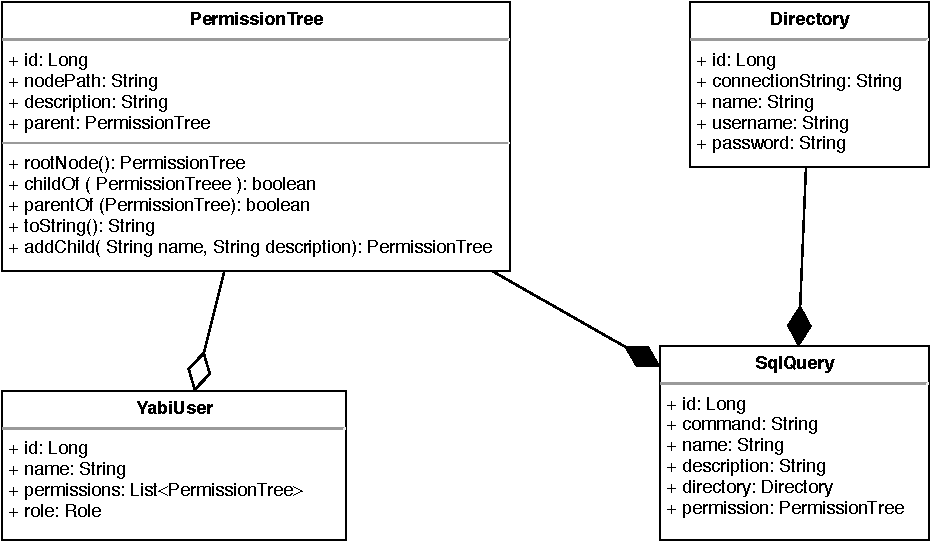
\includegraphics[width=.5\textwidth]{images/diagramas/class}
  \caption{Class diagram}\label{fig:classdiagram}
\end{figure}

\section{Template Sb-Admin-Material}
\section{Multi-Database Support}

Even though the context in which the application described in this document will be primarily accessing Oracle databases, support for other databases was added to broaden its usefulness.

As far as the project for implementing this feature goes, Figure\ref{fig:multidbproj} hopefully describes the process. When a request to run a given Query arrives,

\cleardoublepage
\chapter{Implementation and Results}\label{cha:implementation}

\section{Front-end}\label{cha:implementation:sec:front-end}
\dots

\subsection{Interfacing with Spring Repository}
Because the back-end is mostly implemented using Spring Repositories, which is an abstraction over the persistence of information, many \gls{API} requests are followed by replies that have a general but not consistent \gls{JSON} structure, making it time-consuming to use Typescript's typing capabilities for each and every entity and their Spring Repository structure.

Therefore the motivation behind the development of this architecture is to enable developers to make use of Typescript's typing system when dealing with a Spring Repository default responses and in doing so their \gls{IDE} can show auto-completion suggestions, type-check the code and show possible errors before running the application.

Listing~\cite{code:json} show such a response from \texttt{SqlQueryRepository} that list all elements registered in its database.

Under the key \texttt{\textunderscore embedded}, line 2, there is a single element whose key is the plural version of the entity's name and the value is a list of entities. The \texttt{\textunderscore links} key exposes the actions that can be taken from this resource and \texttt{page} provides information about the current state of the pager.

For most applications, the most interesting part are the elements that make up the \texttt{\textunderscore embedded.sqlQueries} array as it composed of serialized definitions of the back-end models. These definitions also follow the \gls{HATEOAS} pattern of having their relations listed as \gls{URL}s. For example, a \texttt{SqlQuery} is related to one \texttt{Directory},  therefore it can be accessed through the \textbf{/sqlQueries/99/directory} \gls{URL}, made explicit on line 15 and 16.

The common elements between all the implemented repositories are the pager section seen on line 37, the relative links to the listing itself seen on line 25 and the previously stated \texttt{\textunderscore embedded} key that references the element array. Every one of the listed elements contain the self \gls{URL} seen between lines 8 and 11.

Although it is a very declarative to human beings, this \gls{JSON} format is not very machine-friendly due to the ever changing key that references the array of elements. As seen on line 3, \texttt{SqlQueryRepository} uses \texttt{sqlQueries} and other repositories follow suit with \texttt{DirectoryRepository} using \texttt{directories} and \texttt{PermissionTreeRepository} using \texttt{permissionTrees}. This approach is not easily modeled in Typescript. 

With the previous observations it was possible to abstract every repository response into three classes, a \texttt{Repository}, an \texttt{Accessor} and an \texttt{Entity}, enabling the implementation of a generalized repository that is able to interact with Spring's \texttt{PagingAndSortingRepository} in a convenient and typed manner.
Logically a \texttt{Repository} provides access to an array of \texttt{Entity} through the key whose name is define through an \texttt{Accessor}. Figure~\ref{fig:springresponse} provides an overview of how these entities relate.

Throughout this document the term ``hateoas class'' refers to a Typescript class that extends an \texttt{Entity} and a ``normal class'' or ``non-hateoas class'' to be the class that reflects the entities evaluated in the Project section but do not extend \texttt{Entity}. This happens because when the system is accessed by an user, the requests are served by an hand-written endpoint that does not comply with the Repository structure and when it is accessed by an administrator Spring Repositories were used.

\begin{figure}
  \centering
  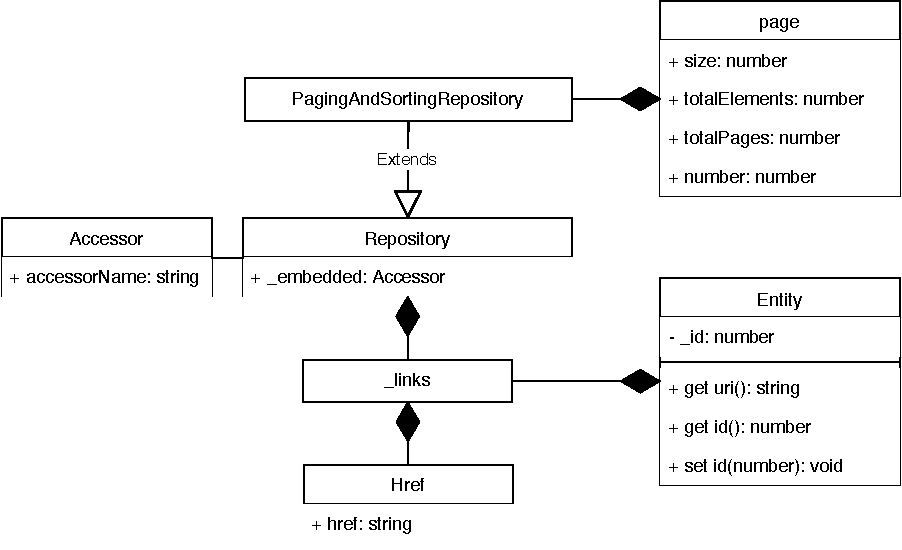
\includegraphics[width=.8\textwidth]{images/diagramas/hateoas_diagram}
  \caption{Class diagram that represents the structure of a Spring Repository response}\label{fig:springresponse}
\end{figure}

\lstinputlisting[float,
caption=DirectoryRepository \gls{HATEOAS} response,
label=code:json
]{images/hateoas.json}

\subsubsection{Entity Class}
This class is typed to accommodate the structure found in the array of elements contained within a repository response, leaving each specification to extend it and add their own fields. It also provide default implementations for \texttt{id} getter and setter and \texttt{uri} getter, that are useful when converting from hateoas classes to non-hateoas classes.

\subsubsection{Accessor Class}
To deal with the fact that the array of persisted elements is found under a key whose name depends on the entity in which the repository provides, the \texttt{Accessor} interface was written.

In its definition, there is only one field, \texttt{accessorName}, that contains a string which can be used to reference the array of persisted elements. Even though this approach functionally works, it compiles and runs, it does not provide the \gls{IDE} with enough information to aid the programmer into navigating the response structure because the value of accessing an object with a key that is unknown in run time is also unknown.

To circumvent this limitation all classes that implement the \texttt{Accessor} interface should also contain a option key whose name is the same one defined in the value of \texttt{accessorName} and its type is an array of entities provided by the repository. With this, the \gls{IDE} is able to auto-complete and type-check the whole response, from repository to individual entity fields.

\subsubsection{Repository Class}
This repository attempts to map Spring Repository response as a whole. In other words, they are the top-most level of the response, mapping the first level of key-values to Typescript types. There are two classes that make up this abstraction, the \texttt{Repository} class that map the \texttt{\textunderscore embedded} and \texttt{\textunderscore links} keys and the \texttt{PagingAndSortingRepository} extension that adds a \texttt{page} key to the mapping.

\subsubsection{Repository Service Class}\label{hateoas:service}
When the previous classes were written to map the \gls{API} responses, their similarities became more evident and the motivation to implement a generic service arose. With this came the \texttt{PagingAndSortingRepositoryService} service that implements \gls{CRUD} interactions with a Spring Repository in a generically-typed manner. These \gls{CRUD} interactions are translated to four functions, \textit{index} that retrieve all entries, \textit{create}, \textit{delete} and \textit{patch} alters a given entry.

Implementation-wise this class is an composed of the three generic elements previously evaluated, \texttt{Entity}, \texttt{Accessor} and \texttt{PagingAndSortingRepository} and its constructor needs a function that return new instances of \texttt{Entity}, an instance of \texttt{Accessor}, the \texttt{HttpClient} service and a string with the address of the remote Spring Repository.

While developing this service, a unexpected behavior was met. When specifying the type of a \texttt{HTTP} request, it did not create a new instance of the received data, which made the behaviors associated to the \texttt{Entity} class and its extensions to not function. This was mitigated by adding the required parameter in the constructor called \texttt{entityConstructor} whose value must be a function that takes no arguments and returns an instance of the repository's entity, then every response follows the pattern of creating a new of such instance and copying all properties from the textual response to it using the \texttt{Object.assign} function.

With all this in place, implementing a service that has no behaviors other than \gls{CRUD} operations is no more than specifying the \texttt{PagingAndSortingRepositoryService} class. Listing~\ref{code:directoryservice} show the implementation of \texttt{DirectoryService}. Note that all it does is extending \texttt{PagingAndSortingRepositoryService}, providing its \texttt{Directory}-specific classes instead of the generic triad and overloading the constructor on lines 21 to 23 so that it can further specify the parent's behavior.

\lstinputlisting[firstline=16, lastline=25, float,
caption=Implementation of the Query model,
label=code:directoryservice
]{frontendlink/layout/directory/directory.service.ts}

\subsection{Component Structure}
When developing the Angular front-end over the \texttt{Sb-Admin-Material} template, it was noted that the example pages that could be accessed by links listed in the left sidebar, seen on Figure~\ref{fig:visible}, were found inside the \texttt{/app/layout} folder. Therefore it made sense to follow this approach and implement \gls{Yabi}'s custom pages in the same place.

In general, each entity have got a folder that contains:
\begin{itemize}
\item A ``model'' file with:
  \begin{itemize}
  \item A class that represents the entity, to be used when retrieving entities depending on the current user.
  \item A class that extends \texttt{PagingAndSortingRepository}, to map Spring Repository responses.
  \item A class that extends \texttt{Entity}, representing the elements contained within the repository response.
  \item A class that extends \texttt{Accessor} that indicates key used to access the list of \texttt{Entity} contained within the repository response.
  \end{itemize}
\item A Service file that extends \texttt{PagingAndSortingRepositoryService}, specifying it for the given entity.
\item The Module file declaring its dialog Components to also be loaded with \texttt{entryComponents}.
\item The Template file that renders a listing with the available entities.
\item A Component file that interacts with the Template and create dialogs.
\item The Style file with rules to correctly render the ``add'' button.
\item A folder with a dialog Component for creating more entries.
\item A folder with a dialog Component for editing an entry.
\end{itemize}

There are some variations to this rule. \texttt{User} Component only has only one dialog that is used to show more information about the current user. \texttt{Query} Component was one of the first components to be developed and it has three dialogs, one for showing more information and the results of running it, one for creating new queries that is not used and a ``form'' dialog that maps a \texttt{Query} to input elements that is used for editing and creating.

\subsection{Components}
Every entity defined in the project section have got a corresponding Angular Component that follows the structure previously defined with a certain degree of freedom. To avoid repeating the common structure previously defined, the particularities of each component in regards to each element will be shown.

Angular services are an abstraction over the remote \gls{API}. In this implementation, almost all resources are provided by Spring Boot's Repository interface, yielding a standard \gls{HATEOAS} reply no matter the entity. Given such repetition, it made sense to implement a common interface through which all Angular Services could inherit and extend the interaction with Spring's \texttt{PagingAndSortingRepository}, therefore  \texttt{UserService}, \texttt{QueryService}, \texttt{PermissionService} and \texttt{DirectoryService} all extend \texttt{PagingAndSortingRepositoryService} and may have added functionalities of their own.

\subsubsection{Login}
% service
\texttt{LoginService} is different than the other services because it does not extend \texttt{PagingAndSortingRepositoryService} and is concerned with providing login functionality and system-wide predicates about the current user or session. The two main predicates are \textit{isAdmin} and \textit{isAuthenticated}, the first is used on templates to hide elements that should not be seen by non-administrative users and the second is run before every request sent to \gls{API} so that the application can redirect to the login page if by some reason the user access a page without first logging-in. It also provides \textit{login} and \textit{logout}, the former saves the username and password combination in the local storage to be used by \texttt{authenticationInterceptor} and requests the \gls{API} route \textbf{/user} for information about the current user; the latter deletes the current user's instance, clears the local storage information and redirects to the login page at \textbf{/login}.

% template
This component came as part of the \texttt{Sb-Admin-Material} and can be seen on Figure~\ref{fig:loginerror}. Mainly, it provides a standard text input for user identification, protected text input for passwords and a \texttt{Login} button that is associated with the component's \textit{onLogin} method. The other \gls{HTML} elements are not bound to any function.

% component
Its Component is very short. It provides a \textit{onLogin} method that in turn call the \texttt{LoginService.login} with the content written in the text inputs. If the login was successful it redirects to \textbf{/query}, otherwise it throws an error saying ``Authentication Unsuccessful''.

\subsubsection{User}
% service
\texttt{UserService} extends \texttt{PagingAndSortingRepositoryService}, specifying it for the \texttt{User} model and provide functions for managing the association between user and permission, listing an user's permissions with \textit{permissions}, creating the relation with \textit{assignPermission} and removing it with \textit{unAssignPermission}. It is worth noting that the process of creating this association involves a \textsc{post} request to the user's permissions address in which the body is composed of line-break separated \gls{URL} links and the header indicates a content type of \texttt{text/uri-list}.

% template
When non-administrative users logs in the application, they are redirected to the \textbf{/queries} page so they can quickly execute one of their use-cases. Figure~\ref{fig:userquerylist} show the page with queries available to the current user. In the top right corner the username is shown to be \texttt{professor} and when clicking the first circle to its right a small pop-up appears with their role. One last thing to note is that non-administrative users such as the one from the figure, do not have access to all screens and buttons. In comparison to Figure~\ref{fig:adminpermisisonnew}, administrators have buttons on the side menu that redirect to \texttt{Directory} and \texttt{User} components, and also a pink round button with an plus sign on the bottom right that enable the insertion of new entries.

These administrative elements are triggered visible though the \textit{isAdmin} method from \texttt{LoginService} and they serve a purely cosmetic function as the back-end denies the execution of administrator functions for standard users.

\begin{figure}
  \centering
  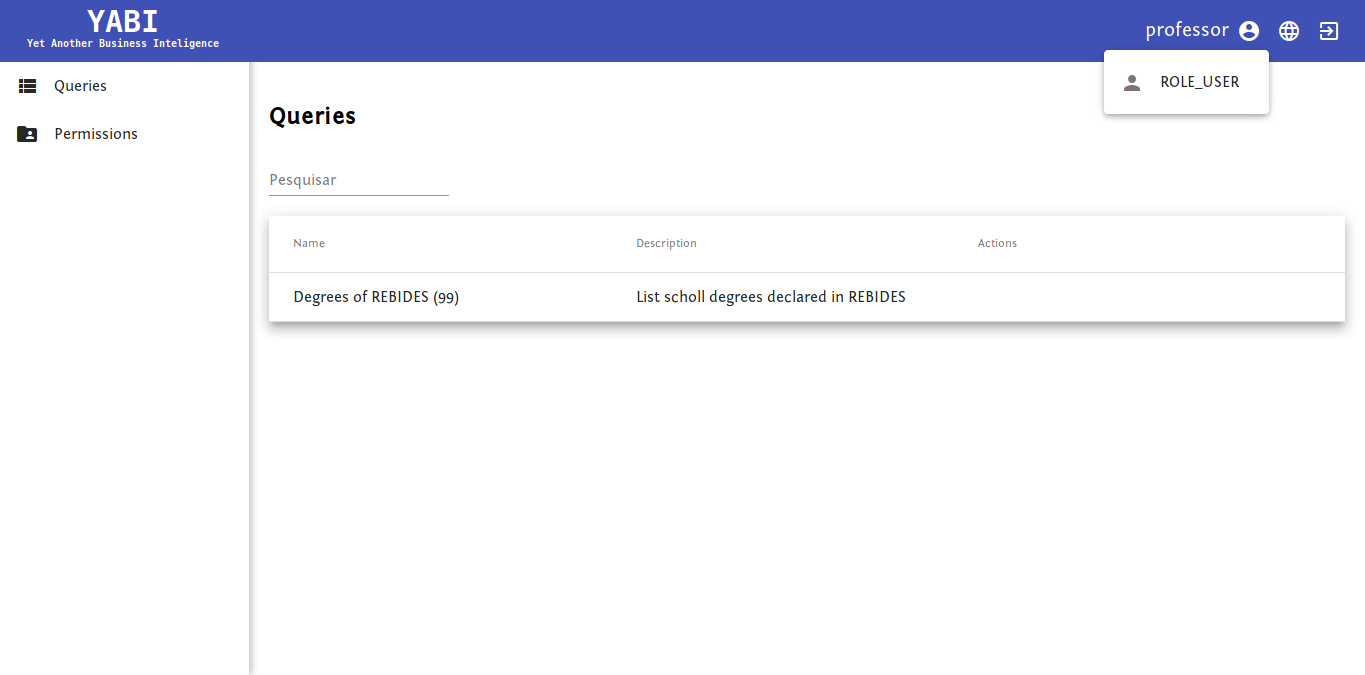
\includegraphics[width=.8\textwidth]{images/screenshots/user/user-query-listing-and-role}
  \caption{Listing of all registered \texttt{Query} for a given \texttt{User} and \texttt{Role} information}\label{fig:userquerylist}
\end{figure}

The use-case of assigning permissions to users is done by administrators at the \textbf{/user} page. The listing itself is very similar to the one seen on Figure~\ref{fig:userquerylist} albeit with two columns, one for the username and the other for role.

As seen on Figure~\ref{fig:adminpermisisonnew}, when a line of the user listing table is clicked, a \texttt{UserShowComponent} dialog appears with a table that lists their associated permissions and possible actions. From there, the administrator is able to remove a user's permission by clicking on the trash can symbol or grant new permissions by choosing one in the drop-down list that says ``Assign new Permission'' and clicking on the adjacent plus symbol.

\begin{figure}
  \centering
  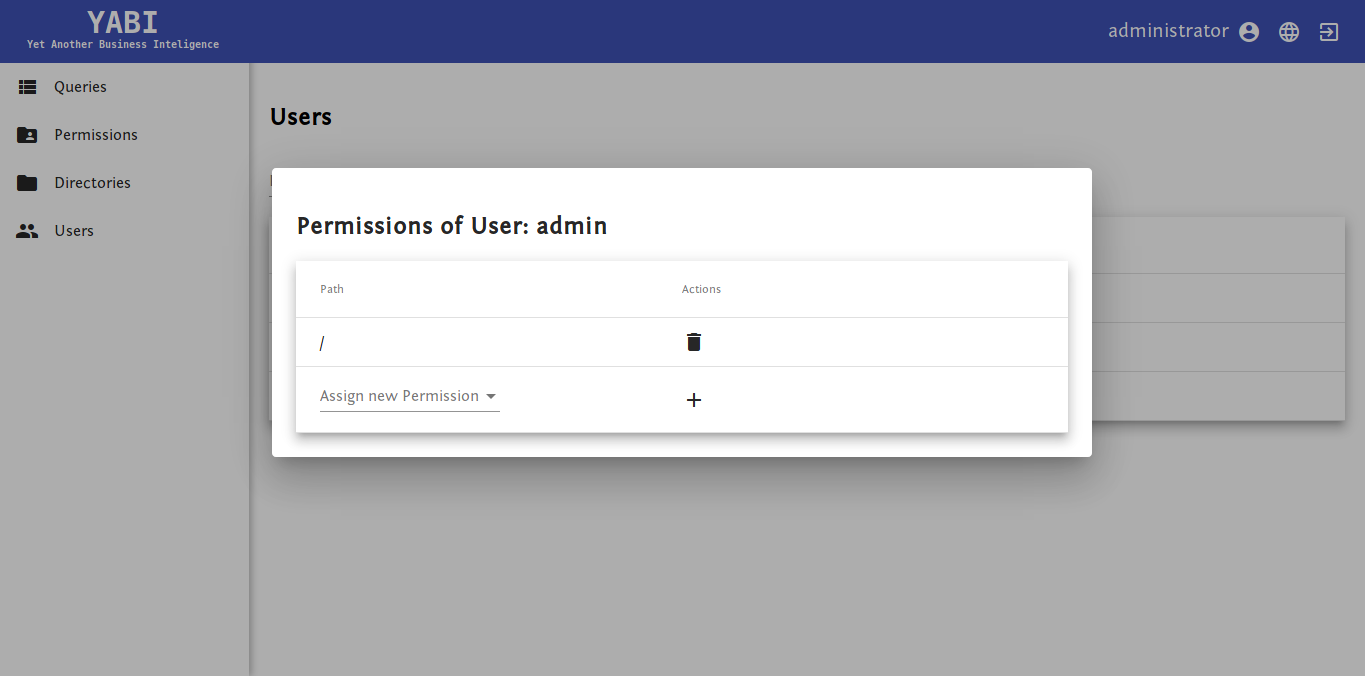
\includegraphics[width=.8\textwidth]{images/screenshots/user/admin-permission-new}
  \caption{Dialog for assigning a new \texttt{Permission} to a \texttt{User}}\label{fig:adminpermisisonnew}
\end{figure}

% model
The \texttt{HateoasUser} class extends the generic \texttt{Entity} with attributes that compose the back-end implementation of the user. Interestingly enough, because back-end class is written to fit within the Spring Framework authentication mechanism, it has some unused back-end specific attributes added to what was initially defined in the project, these include the attributes \texttt{enabled}, \texttt{authorities}, \texttt{password} (left empty), \texttt{accountNonExpired}, \texttt{accountNonLocked} and \texttt{credentialsNonExpired}.

\subsubsection{Query}
% service OK
\texttt{QueryService} is quite different when compared with other services because it implements the standard features found in \texttt{PagingAndSortingRepositoryService}. This is because it was one of the first services to be developed and the need for a common interface was not yet evaluated. To keep compatibility, with the current modules, the function names and signatures were kept intact but their implementation makes use of \texttt{HateoasQueryService}, which does extend the common service. Regarding the other services, this one provides a different behavior for \textit{index} that requests the queries in which the current user have access to. Lastly there is the \textit{run} method which is specific to this service, requesting the \gls{API} into running a query and yielding its results.

% template
Shown on Figure~\ref{fig:userquerylist}, the \textbf{/query} page presents a table that list queries in regards to their\texttt{Name}, \texttt{Description} and \texttt{Actions}. The last one being dependent on the user role. If accessed by an administrator there are two icons, a pen that when clicked raises a editing dialog and a trash can that deletes the query; if accessed by an user, as seen on the figure, this column is not rendered. Create and edit dialogs are similar to those made for the Directory entity but of course the form fields match the attributes of \texttt{query} model.

% component
\texttt{QueryComponent}, like the others, interacts with the listing template by handling the actions that can be done on this page. Clicking on the list element is bound to \textit{onQueryShow} which raises the \texttt{QueryShowComponent} dialog; the add button and the edit action raises \texttt{QueryFormComponent} dialog with different data, creating a new query pass no information to the dialog and editing passes the clicked query element. \texttt{QueryFormComponent} is smart enough to take different actions depending on its input so that a new query gets persisted and an already existing query it patched.

% dialogs & module - nao esquecer o databaseReader
When a table element is clicked, the dialog seen in Figure~\ref{fig:queryprerun} is shown. It presents to the user the query's \texttt{Name}, \texttt{Description} and \texttt{Permission} alongside two button on the lower right, ``Run'' and ``Download''. The former invoke an \gls{API} method on \textbf{/runQuery/\{id\}} to execute it, retrieve the results and display them in a table similar to what is shown in Figure~\ref{fig:querypostrun}; the latter does the same but in the end prompts the user to save a \gls{csv} file with the results. 

% model
Because queries must be filtered in regards the current user's permissions, \texttt{QueryService} requests the \gls{API} on a custom controller located at \textbf{/queries} that does not comply to the \gls{HATEOAS} pattern, inducing the creation of two models, one that extends the common \texttt{Entity} class to map eventual \gls{HATEOAS} responses and the other that is on par with the response from \textbf{/queries}. It is interesting to note that \gls{UI} elements are build around the latter model because it enables one single screen to serve both user roles, the conversion from \texttt{HateoasQuery} to the non-hateoas version is straight forward given that \texttt{Query} is simpler with no nested attributes.

\begin{figure}
  \centering
  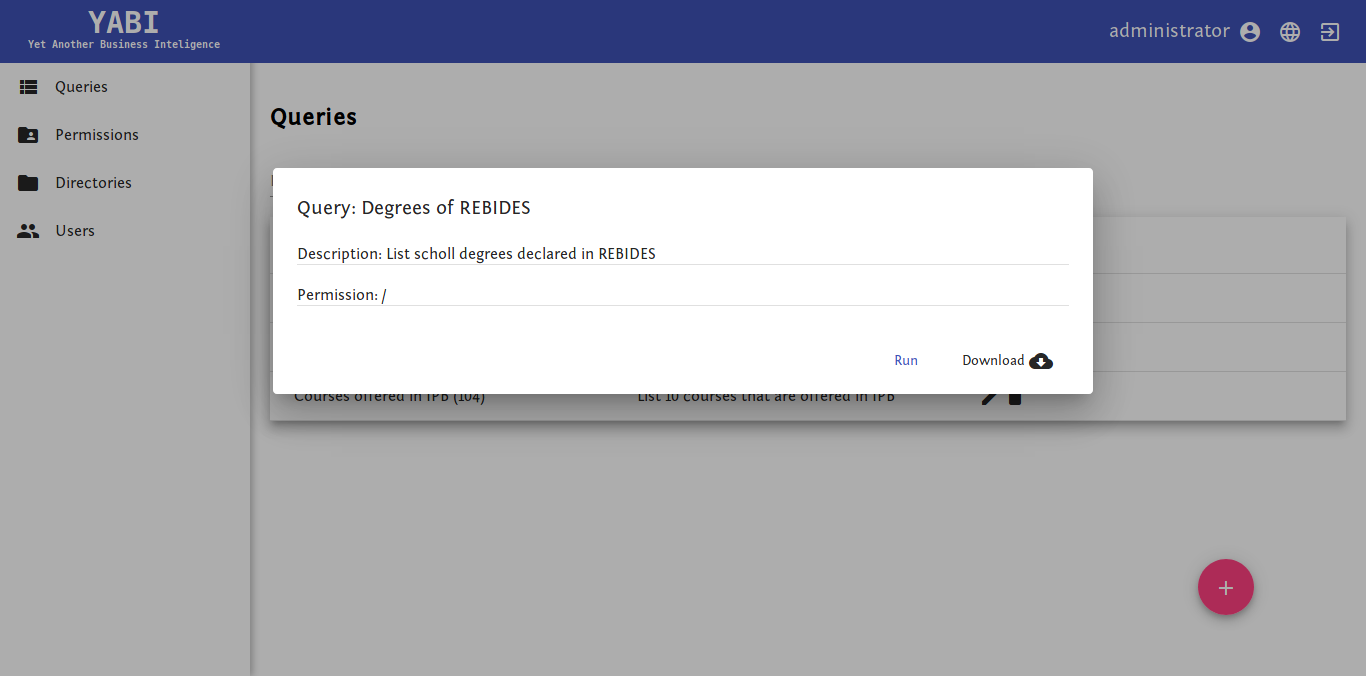
\includegraphics[width=.8\textwidth]{images/screenshots/query/query-pre-run}
  \caption{Dialog for running a \texttt{Query}}\label{fig:queryprerun}
\end{figure}

\begin{figure}
  \centering
  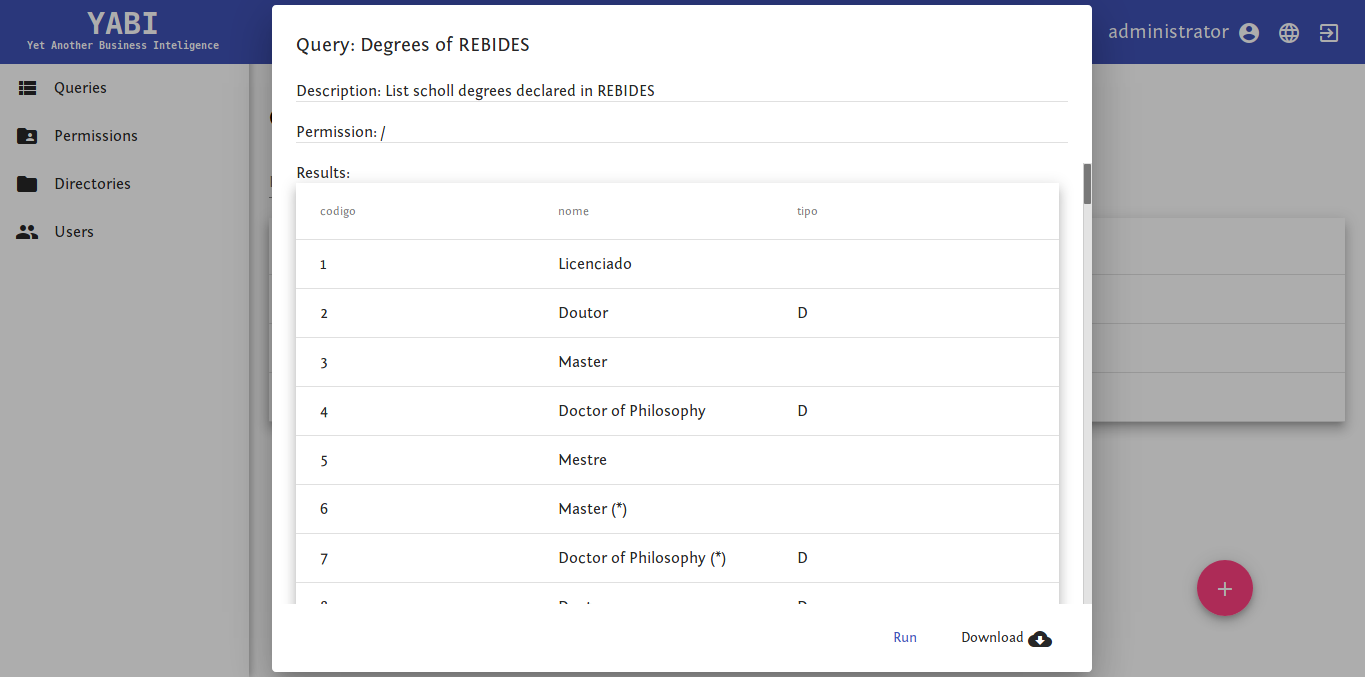
\includegraphics[width=.8\textwidth]{images/screenshots/query/query-post-run}
  \caption{Dialog for running a \texttt{Query} after it was executed}\label{fig:querypostrun}
\end{figure}


\subsubsection{Permission}
% service OK
\texttt{PermissionService} have only two particular methods, one for requesting the current user's permissions called \textit{userIndex} and a custom implementation of \textit{delete} which uses \gls{Yabi}'s custom implementation in \textbf{/delete}.

% template
% dialogs & module
The screen that lists the available permissions is also similar to that seen on Figure~\ref{fig:userquerylist}, although its table has different columns, \texttt{Path}, \texttt{Description} and \texttt{Actions}, with this last one visible only to administrators. The action column has two icons, a plus sign that indicates the creation of a new child permission and a trash can for deletion. Clicking the row raises a dialog for editing its description. The key difference between this entity and the others when it comes to creating a new entry is that because permissions follow a hierarchy, the first step towards creating a new entity is to choose its parent permission and clicking on the plus sign on its row. Figure~\ref{fig:permissionnew} presents the dialog raised when doing so, Note that it shows the parent permission's canonical path alongside its description.

\begin{figure}
  \centering
  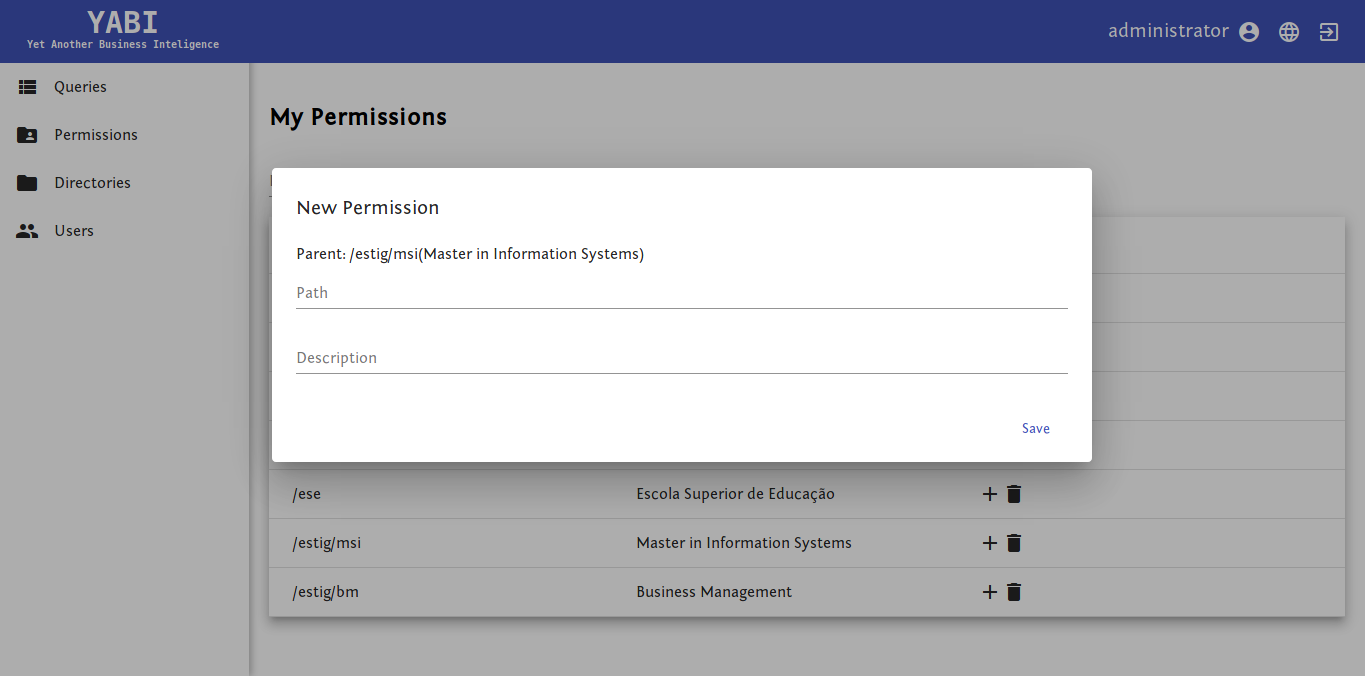
\includegraphics[width=.8\textwidth]{images/screenshots/permission/permission-new}
  \caption{Dialog for creating a new \texttt{Permission}}\label{fig:permissionnew}
\end{figure}

% component
The main component is bound to listing the available permissions. Similar to \texttt{QueryComponent}, this page serves both user roles the same way but contrary to it, \texttt{HateoasPermission} is used as the base model. This is because \texttt{Permission} class implements the \textit{toHateoas} method and even thought they share much of the same fields, the converted \texttt{HateoasPermission} is generated with a undefined \gls{URI} attribute. There are two sub-components, \texttt{PermissionFormNewComponent} and \texttt{PermissionFormEditComponent}. As the name suggests, they interact with the user and \gls{API} when creating and editing permissions. One interesting thing to note is that when persisting a new permission, the \textit{onSubmit} method appends the separator character to the path.
% model

\subsubsection{Directory}
% service OK
Lastly there is the \texttt{DirectoryService} whose implementation is nothing more than the proper extension of \texttt{PagingAndSortingRepositoryService}. In fact, it is so small that it was used as an the minimal usage example in Section~\ref{hateoas:service}.

% template
The directory listing page is only accessible to administrative users, which made its implementation very compliant to  \gls{HATEOAS} pattern used by Spring Repository. It uses the same listing presentation shown in Figure~\ref{fig:userquerylist} with columns for \texttt{Name}, \texttt{Connection String}, \texttt{Username}, \texttt{Password} and \texttt{Actions}, showing the icon of a trash can that signifies deletion. Clicking the row itself raises the \texttt{DirecotryFormEditComponent} in a dialog, allowing the administrator to edit the clicked Directory.
Figure~\ref{fig:dirnew} shows the dialog used to create a new Directory, it is composed of one textual input per model attribute and a ``Save'' button on the lower right corner. The previously \texttt{DirecotryFormEditComponent} shown on Figure~\ref{fig:diredit} share the same structure but with inputs filled with values from the Directory being edited.

\begin{figure}
  \centering
  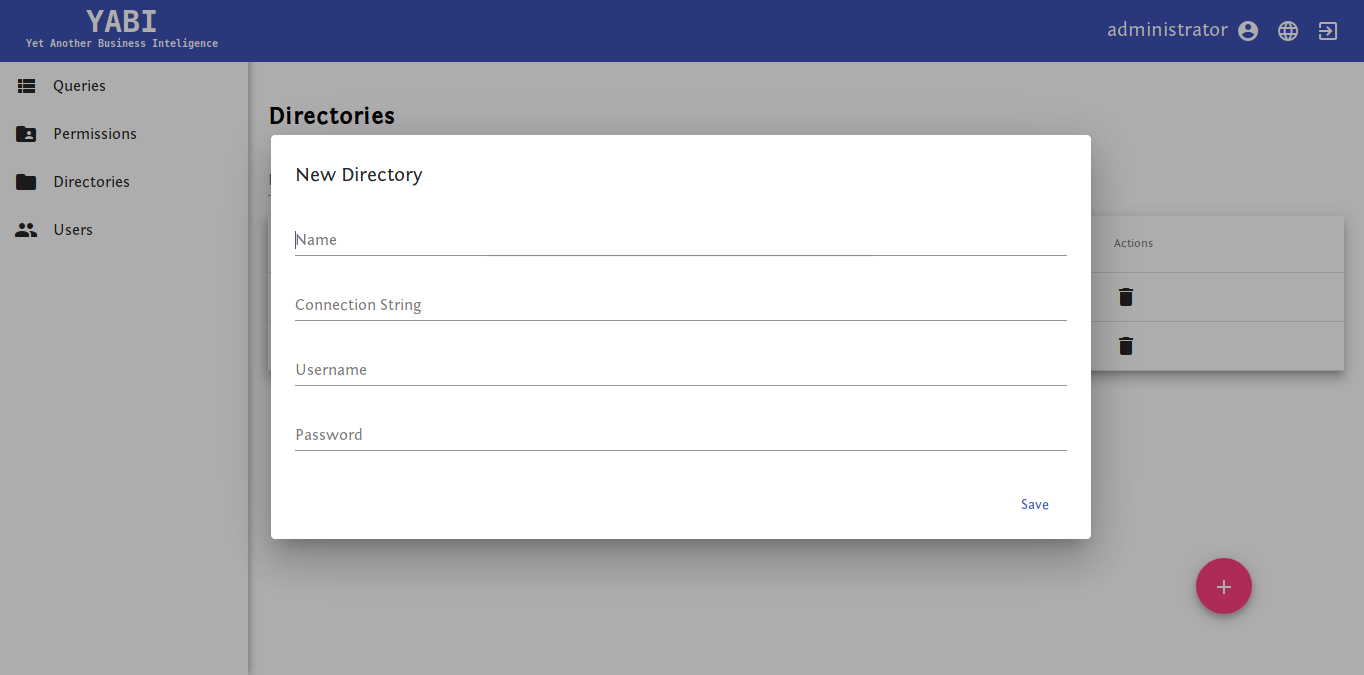
\includegraphics[width=.8\textwidth]{images/screenshots/directory/directory-new}
  \caption{Dialog for creating a new \texttt{Directory}}\label{fig:dirnew}
\end{figure}

\begin{figure}
  \centering
  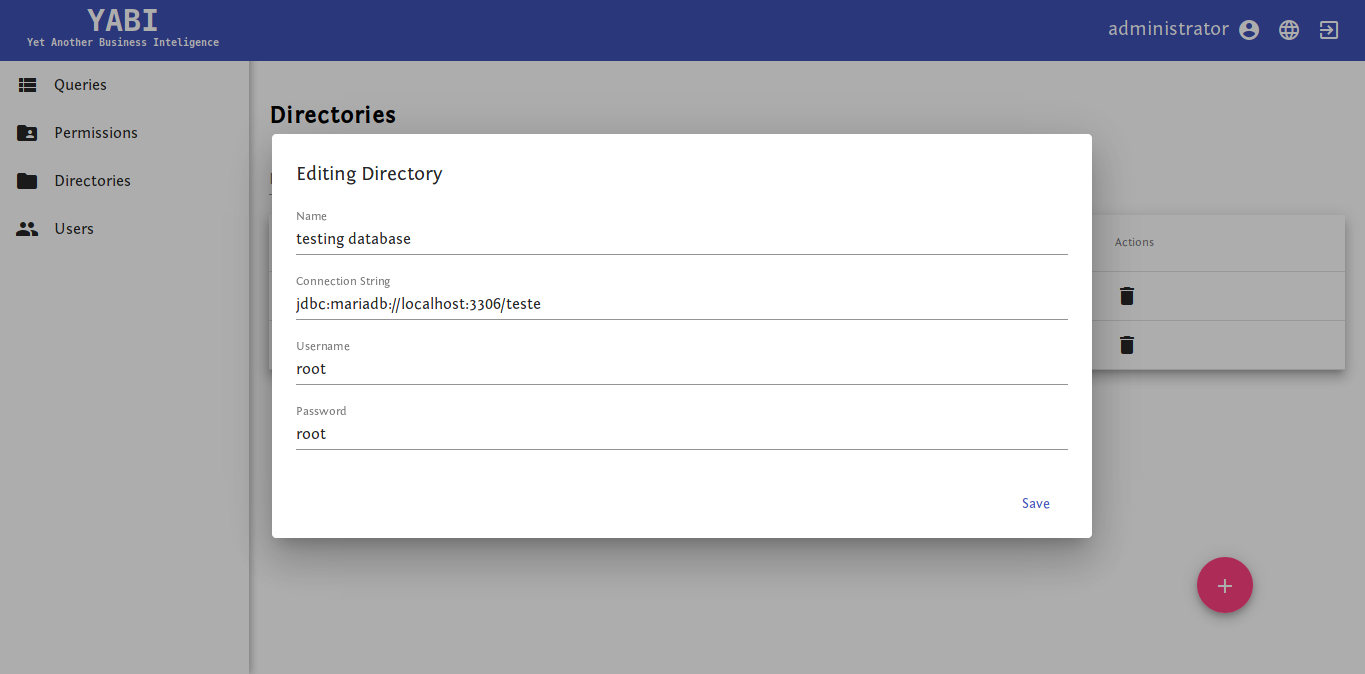
\includegraphics[width=.8\textwidth]{images/screenshots/directory/directory-edit}
  \caption{Dialog for editing an existing \texttt{Directory}}\label{fig:diredit}
\end{figure}

% component
The component implementation is very straight forward with the listing page fetching elements using the \texttt{DirectoryService} and binding the buttons to trigger their respective behavior. The plus button that indicates the creation of a new directory is bound to method \textit{onDirectoryNew}, clicking the row to \textit{onDirectoryShow} and the trash can to \textit{onDirectoryDelete}. The first two delegate the interaction to another components that are displayed in a dialog. 

% model
Being accessible only to administrative users means that the whole \gls{API} interaction can be done through Spring Repositories. This means that the only model being exchanged is that of \texttt{HateoasDirectory} that extends \texttt{Entity} and nothing more.

\subsection{Generic Form Control Builder}
Every form used for editing and creating new entries follow the pattern of providing a text input for each attribute of the model. To reduce repeated code for generating a \texttt{FormGroup} with the given model's attributes the function \textit{genericFormControl} was implemented.

What it does is take an instance of any object and a optional list of attributes to ignore and assign to an object every attribute name evaluated from calling \texttt{Object.keys} on the instance with a new \texttt{FormControl} with that attribute's value, skipping the attributes found the ignore-list. In the end, return a new \texttt{FormGroup} with such object.

This way, when creating a form for editing a model, this function will return all the control with values already filled, ready to be bound to a form in the template definition. Also, when creating a new entry, the resulting \texttt{FormControl} edited by the user will have matching fields with the model, allowing for fewer conversion between what is inputted and what is sent to the \gls{API}.

\subsection{Temporal Caching Repository}
Because \texttt{PermissionService} is by a few different classes and because permissions are not frequently inserted in the system, it was found that not many \gls{API} requests are necessary during a session. Therefore a temporal caching system was developed on top of the existing \texttt{PagingAndSortingRepositoryService} so that in a configured time span, the service will not actually request the \gls{API} but instead provide elements that are kept in memory. Once the time expires, the local cache is considered invalidated and a new \gls{API} is issued.

Implementation-wise it intercepts the actual \textit{index} method saving a local copy of the response in memory. When a request to \textit{index} happens within the time frame specified in \texttt{SharedModule.serviceCacheExpirationTime}, it returns a observable of its local cache. The cache itself is implemented as an array of elements in which the service is providing.

\subsection{Error Handler}
By default, every Angular app provides a \texttt{ErrorHandler} that simply writes to the browser's console. However users must be notified when an error happen so that they can either take action or contact the IT department if it persists. To do so, \texttt{ErrorHandler} was extended into \texttt{SnackBarErrorHandler}, which as the name suggests creates a snack bar element with the error message, and was provided in the root module so that any uncaught error in the application is handle by it, effectively replacing the standard \texttt{ErrorHandler}. Figure~\ref{fig:loginerror} show the visual element that is created when an error occurs.

\begin{figure}
  \centering
  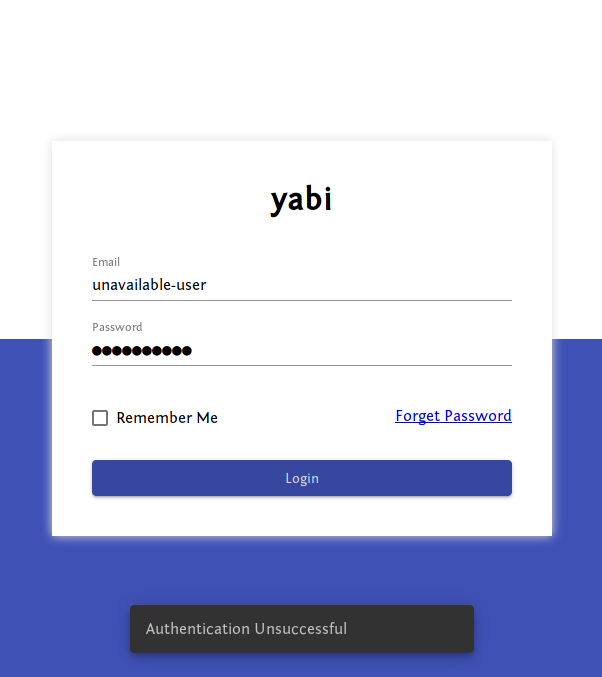
\includegraphics[width=.7\textwidth]{images/screenshots/login-error}
  \caption{Login screen with a authentication error caught by the \texttt{SnackBarErrorHandler}}\label{fig:loginerror}
\end{figure}

\subsection{authenticationInterceptor}
Because the back-end handle requests in a stateless fashion, authentication information must be sent alongside every \gls{API} request.

This was achieved by creating the \texttt{authenticationInterceptor} class that implements the \texttt{HttpInterceptor} interface and overrides the method \textit{intercept} by injecting the \texttt{Authorization} header to requests that addressed to the \gls{API}.

There are some occasions that require different or no treatment. If the request is not destined to \gls{Yabi}'s \gls{API}, the request is processed as usual and if the user is not authenticated the application redirects to \textbf{/login}, prompting the user to login again.

\subsection{apiEndpoint}
Though as a Service, this class is declared in the app's root module and therefore can be injected into any component. It's job is to abstract all the endpoints available in the interface either through constant strings that point to repositories or functions that assemble an address for an entity given it's id.

Some example endpoints include the \texttt{PERMISSIONS} attribute that refers to the \gls{API}'s \textbf{/permissions} that return all the permissions associated to the current user; \texttt{ADMIN\textunderscore PERMISSIONS} referring to \textbf{/permissionTrees}, which is the interface managed by a Spring Repository and lastly there is the \textit{USER\textunderscore PERMISSION} function that takes in an user id and a permission id and returns the address that represents the association between them so it can be, for example, deleted.

\subsection{Shared Module}
The \texttt{SharedModule} is a class that is imports and exports all Angular Material directives. This was done to speed up development time, removing the necessity of importing each specific module when it is needed. The performance impact of including all of Angular Material was not found to be noticeable during development when compared to building it with \gls{AoT}.

Another use of this module is providing application-wide constants. There are three static attributes, \texttt{debounceTime} which is the time in milliseconds between keystrokes to consider that the user has finished typing their search term; \texttt{serviceCacheExpirationTime} which is the lifespan of the information kept in a \texttt{CachedPagingAndSortingRepositoryService} and lastly, \texttt{apiBase}, which is the base \gls{API} address.

\subsection{Security Concerns}

When a user logs-in the application, their username and password is stored as a base64 string in the local storage. Should the application be compromised with attacks such as \gls{XSS}, the injected code is able to access the user's credentials.

Another concern is in regards to the stateless nature of the back-end, requiring the credentials to be sent with every request. If the connection is not encrypted, credentials will be sent as plain base64 encoded string, which is easy to spot and decode. In the front-end this can be mitigated with \gls{HTTPS} encryption and in the general view a token could be exchanged to avoid having the credentials being frequently sent to the \gls{API}.

\section{Back-end}\label{cha:implementation:sec:back-end}
\dots

\subsection{Entities}
Following the class diagram in Figure~\ref{fig:classdiagram} and their relations, classes were created and properly annotated with so that \gls{JPA} is able to properly generate a relational model. Hence the \texttt{Entity} annotation is present in all classes.

Listing~\ref{code:sqlquery} presents the implementation of the Query model defined in Section~\ref{model:query}, it servers as an overview into other model implementations as it shares much of the common features but also adds some of its own.

Lines 1, 2 and 5 are provided by the Lombok package as discussed in Section~\ref{tech:lombok}, instructing the creation of constructor and other common methods during compilation. All models make use of \texttt{@Data} and \texttt{@NoArgsConstructor} annotations and all but \texttt{PermissionTree} uses \texttt{@AllArgsConstructor}.

In regards to \gls{ORM}, \texttt{@Entity} annotation in line 3 is the entry-point through which \gls{JPA} evaluates what classes are meant to be taken into account when building the relational model.
In general, some attributes need don't need to be declared as they are correctly inferred but in some cases it is desired to configure the generated database, \texttt{@Column} annotation on line 11 changes the default behavior so that the length of the corresponding \texttt{varchar} field in the table is able to hold larger amounts of characters; The other models, \texttt{YabiUser} \texttt{PermissionTree} and \texttt{Directory} make extensive use of \texttt{@Column} to specify columns that shouldn't have repeated values.

Relation between entities are made though \texttt{@OneToOne}, \texttt{@ManyToOne} and \texttt{@ManyToMany} annotations.
The first two represents single value association between entities, however, they represent different semantics and where the foreign key will be created.
\texttt{@ManyToOne} indicates that the foreign key will stay in the table in which this model is mapped to, \texttt{@OneToOne} makes no distinction, leaving for the \gls{ORM} back-end implementation to decide.
Line 17 is declaring that more that one instance of \texttt{SqlQuery} may reference a single \texttt{Directory} and that \texttt{SqlQuery} will hold the foreign key to \texttt{Directory}.
\texttt{@ManyToMany} represents a collection of associations, here used to associate \texttt{YabiUser} to \texttt{PermissionTree} so that many users can have many, overlapping, permissions. One possible parameter to \texttt{@ManyToMany} is the \texttt{FetchType}, instructing the \gls{ORM} engine to retrieve the associated entity only when it is accessed or together with its parent is retrieved.

\texttt{@JoinColumn} annotation is a general purpose configuration for relational fields, in line 18 and 22 it's used to configure the name in which the column will be called and whether it can have no specified value.

\lstinputlisting[firstline=22,float,
caption=Implementation of DirectoryService,
label=code:sqlquery
]{listings/SqlQuery/SqlQuery.java}

The remaining entities follow a similar pattern in it's implementation.

\subsection{Spring Configuration}
In order for Spring Framework to stay out of the way as much as it can and allow developers to focus on the implementation of business functionalities, it makes many assumptions about how its components interact, however, at some point the application being developed grow some needs that conflict with Spring defaults. When this eventually happens, which was the case with \gls{Yabi}, developers can override some of Spring's default behavior by implementing specific interfaces. More on Spring can be found in Section~\ref{concept:spring}.

This section presents Spring configurations that took place so that \gls{Yabi} is able to work as expected.

\subsubsection{Security}
\gls{Yabi}'s security model uses a directory server to authenticate and a relational database to load user roles and execute authorization checks. Because this is a stateless application, every request follows the steps shown in Figure~\ref{fig:authseq} before being executed by the controllers.

Authentication is done through a anonymous bind to a \gls{LDAP} server, Section~\ref{impl:ldap} goes through the Spring configuration necessary to make it work and Section~\ref{impl:detailsmapper} explains how the roles are loaded into the Sprig Security's \texttt{UserDetails} object.

In regards to authorization, there are two possible roles in which a use must be assigned to, either \texttt{ADMIN} or \texttt{USER}. With this, non-administrative resources are simply not dependent on the user's role therefore accessible to all users, meanwhile, administrative resources are explicitly marked to be accessible by users whose role is \texttt{ADMIN}, more on this in Section~\ref{impl:admres}.

Figure~\ref{fig:authseq}, presents in a general view the steps taken to authenticate and load an user's details. It is infeasible to model the whole of Spring Web and Spring Security as it is quite a extensive feature and it is out of the scope of this report, therefore it was abstracted into fewer elements, namely \texttt{WebSecurity} entity representing the objects that gets built by the configuration shown in Listing~\ref{code:authblock}, the \textit{authenticate} message is abstracting Spring's authentication provider voting system, \texttt{LDAP AuthenticationManager} entity representing \gls{LDAP}'s \texttt{AuthenticationProvider} and \textit{anonymous bind}, as the name implies is the authentication that takes place in the directory server.

The main point of Figure~\ref{fig:authseq} is to show that once the bind takes place in the \texttt{LDAP AuthenticationManager}, the library requests an object that implements the \texttt{UserDetailsContextMapper} to populate it's newly created \texttt{Authentication} object with business-specific information in the form of a \texttt{UserDetails}. In this case \texttt{YabiUserDetailsManager} is chosen by Spring's dependency injection mechanism and it provides an instance of \texttt{YabiUser}, which implements \texttt{UserDetails} interface, that is retrieved from \gls{Yabi}'s database.

\begin{figure}
  \centering
  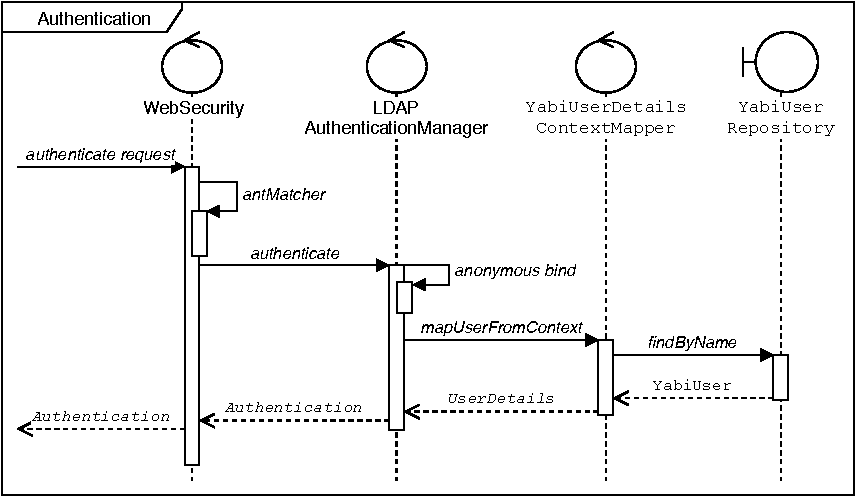
\includegraphics[width=.9\textwidth]{images/diagramas/authentication}
  \caption{Authentication Sequence Diagram}\label{fig:authseq}
\end{figure}


\subsubsection{Admin Resources}\label{impl:admres}
Not all endpoints are freely accessed to all users because they involve possibly destructive interactions with the information contained in the system. In this implementation, non-administrative users get their information through custom \texttt{RestController} that expose fewer functionalities and administrative users may directly request the repositories. Repositories are further discussed in Section~\ref{impl:repos}.

Suffice to say that certain endpoints require the user to be authenticated and to have an administrator role. Listing~\ref{code:authblock} is the configuration that enforces this statement.

The call to \texttt{antMatchers} in lines 9, 11 and 13 works by specifying a list of \gls{HTTP} paths and applying some definitions or restrictions whenever an incoming request is found to match a string pattern. In this specific case, all requests to repositories are eligible to continue being processed only if the \texttt{hasRole} rule evaluates to true.

Line 13 is protecting the \textbf{/permission} endpoint from being requested with a \gls{HTTP} \textsc{delete} verb.
Lines 8 and 14 declare that all \gls{HTTP} requests are to be authenticated.

\lstinputlisting[firstline=39, lastline=55, float,
caption=HttpSecurity configuration,
label=code:authblock
]{listings/Configuration/SecurityConfiguration.java}

\subsubsection{\gls{CORS} Mapping}

Because \gls{Yabi} is a web \gls{API} and a front-end application, it is necessary that both parties can interact but due to security reasons, most browsers implementations block \gls{AJAX} calls if the remote server does not explicitly add the current domain to it's response header.

In Spring, specifying allowing domains to access it's resources is done by implementing the \texttt{WebMvcConfigurer}, overriding the method \textit{addCorsMapping(CorsRegistry)} and calling \textit{allowedOrigins} on it's parameter. The method \textit{allowedOrigins} takes a list of stings that contain valid \gls{URL} addresses.

\gls{Yabi} configures this using the \texttt{application.properties} file under the key \texttt{yabi.web.allowedOrigins}, allowing for a centralized configuration.

\subsubsection{\gls{LDAP}}\label{impl:ldap}

Following the authentication specification in Section~\ref{proj:auth}, Listing~\ref{code:ldapauth} presents the configuration that implements the desired behavior.

\lstinputlisting[firstline=57, lastline=66, float,
caption=LDAP Authentication Configuration,
label=code:ldapauth
]{listings/Configuration/SecurityConfiguration.java}

In this configuration, \texttt{AuthenticationManagerBuilder} is a class used by Spring in it's security pipeline. It comes with built-in support for \gls{LDAP}, \gls{JDBC} and in-memory authentication mechanisms; line 4 is declaring \gls{LDAP} authentication to be used.

Line 5 is considered important because it is mapping a custom details context mapper to the authentication pipeline. What this does is to provide a hook in the authentication pipeline to allow explicit customization of the user object after it is authenticated. The given mapper, \texttt{YabiUserDetailsContextMapper} retrieves the authenticated user's instance of \texttt{YabiUser}.

Lines 6 to 9 configure the connection to the remote directory service, including it's address and what to bind with.

\subsubsection{User Details Context Mapper}\label{impl:detailsmapper}
Often times a directory service is used as an authentication mechanism. Applications issue an anonymous bind request to the server passing their user's credentials and if properly found and matched, a boolean value is returned, however, applications often has information about the user that must be sent accessible to other parts of the framework. To do so, Spring Security utilizes this interface to retrieve a \texttt{UserDetails} instance that gets injected into the commonly accessible \texttt{Authentication} interface.

For this application, a new implementation of the \texttt{UserDetailsContextMapper} interface is provided, \texttt{YabiUserDetailsContextMapper} returns an instance of \texttt{YabiUser}, which implements said \texttt{UserDetails} interface and adds \gls{Yabi}-specific attributes, enabling other parts of the system to query the current user's related information such as their role, \texttt{PermissionTree} and name. More information about the \texttt{YabiUser} class is found in Section~\ref{model:user}.

\subsection{Custom Controllers \& View Models}
\texttt{@RestController} is a Spring Web annotation that enables a given class or method to handle \gls{HTTP} requests. In essence it is a combination of two other annotations, the \texttt{@Controller}, which is what trigger the framework into considering the class as a possible resolver of  \gls{HTTP} requests and \texttt{@ReponseBody}, that wraps the method call into a response body. In simple cases the returned Object is mapped to a \gls{JSON} string.

Because the \texttt{PermissionTree} class contains a reference to it's parent, and the root references itself, there was a need to circumvent a infinite loop during it's \gls{JSON} serialization. To do so, rather simple and 
serializable classes whose role were to convey information to the front-end were written, namely, \texttt{SqlQueryViewModel}, \texttt{PermissionTreeViewModel} and \texttt{YabiUserViewModel}.

To accommodate the special handling of \texttt{PermissionTree} model and provide some custom functionalities, the following custom controllers were implemented: \texttt{SqlQueryController}, \texttt{PermissionTreeController} \texttt{YabiUserController} and \texttt{DatabaseReaderController}. When it comes to providing entities in function of the current user's permissions, the general implementation was done by adding a custom method to repositories that enables them to retrieve elements based on their entity's permission \texttt{nodePath}. This is further explained on Section~\ref{impl:repos}. Listing~\ref{code:queries} show the implementation of endpoint \textbf{/queries} that retrieves \texttt{SqlQuery} elements that are associated to the current user, note on Line 8 the retrieval of all elements whose permission \texttt{nodePath} starts with the user's permission \texttt{nodePath} and on Line 9 the instantiation of a non-recursive, serializable \texttt{ViewModel}.

\lstinputlisting[firstline=27,lastline=39, float,
caption=\textbf{/queries} endpoint implementation,
label=code:queries
]{listings/SqlQuery/SqlQueryController.java}

\subsubsection{DatabaseReaderController}
The retrieval of information contained in a remote database is exposed through the \textbf{/runQuery/\{id\}} address. Breaking the \gls{REST} convention, the interpolated \texttt{id} argument is a number that refers to a persisted \texttt{SqlQuery} class. When this controller is properly requested, it first validates if the requesting user may run it by finding at least one permission associated to the current user that is either higher or equal to that in which the \texttt{SqlQuery} is associated to and calls \texttt{DatabaseReader.runQuery} with the \texttt{SqlQuery} in question.

The method \textit{runQuery} in turn retrieves the associated \texttt{Directory} from the repository and with its credentials, it makes a \gls{JDBC} connection and executes the query command. Lastly the resulting \texttt{ResultSet} is completely read and interpreted into a matrix of strings which is then returned to the controller and finally is useed to answer the \texttt{API} request.

\subsubsection{PermissionTreeController}
Because of it's tree-like nature, once a \texttt{PremissionTree} is deleted, all of it's child nodes need also to be removed. However, because it reference its parent but not its children, leaving the \gls{RDBMS} to execute a cascading delete would delete every parent permission untill the root node.
Therefore \texttt{PermissionTreeController} implements a custom a delete that cascades through its children. It is bound to a \textsc{delete} \textbf{/pemrission/\{id\}}, \texttt{id} being the identifier of the permission to be deleted.

It is implemented by first retrieving the permission whose id was specifies in the \gls{HTTP} request, retrieve all of its children with the custom repository method \textit{findAllByNodePathStartingWith} and sequentially deleting all permissions found and lastly delete the permission itself.

One restriction is that the root node can never be deleted. Therefore, before executing the before-mentioned steps, the permission to be deleted is matched with the root node, if it does, the operation is aborted with an error.

\subsubsection{YabiUserController}
To provide the front-end with information about the current user, \texttt{YabiUserController} replies to \textsc{get} requests on the path \textbf{/user} with information contained inside the \texttt{Authentication} that was generated during the user's authentication procedure and thus avoid reaching out to the database a second time.

\subsubsection{SqlQueryController}
\texttt{SqlQuery} is one of those entities that are related to the current logged-in user. In other words, administrators may see all registered \texttt{SqlQuery} and users see only those which they can run, Therefore \texttt{SqlQueryController} was created.

It has only one method that replies to \textsc{GET} requests to \textbf{/queries} endpoint with a list of \texttt{SqlQueryViewModel}. Implementation-wise it returns a list containing every \texttt{SqlQuery} found in the database by calling \texttt{SqlQueryRepository.findAllByNodePathStartingWith} for every permission associated to the current \texttt{YabiUser}.

\subsection{Spring Repositories}\label{impl:repos}
\texttt{PagingAndSortingRepository} were created for all entities evaluated during the project evaluation phase.
The \texttt{Directory} entity whose did not require any changes in regards to what Spring already provides and won't be discussed.
The remaining entities had their repositories augmented with functionalities presented below.

\subsubsection{YabiUserRepository}
After binding in the directory service, \texttt{UserDetailsContextMapper.mapUserFromContext} is used to fill an instance of \texttt{Authentication} class with business data. In \gls{Yabi}'s custom implementation, this data comes from a relational database that reflect \texttt{YabiUser} objects.

Because the method \textit{mapUserFromContext} uses the username as a key to retrieve information, \texttt{YabiUserRepository} had to be augmented with a new method to do just that. Therefore the following declaration was added:\\
\texttt{YabiUser findByName(String username);}

\subsubsection{PermissionTreeRepository}
When the system needs to validate an action or filter information depending on a permission, it retrieves all of its child permissions. Because this action is frequently used, this repository had also to be augmented.

In this case, the method signature used was as follows:\\
\texttt{List<PermissionTree> findAllByNodePathStartingWith(String~nodePath);}

\subsubsection{SqlQueryRepository}
When an user request a list of queries that they can execute, the system must retrieve from the relational database all queries in which the permission is a child of the user's permission. Again, this repository had to be augmented.

This was accomplished by using the following method interface:\\
\texttt{List<SqlQuery> findByPermissionNodePathStartingWith( String~nodePath );}

\subsection{Multi-Database Support}
Paraphrasing Requirement~\ref{req:multidb}, the application must be able to retrieve information from the institution's database. However, because it has many in-house applications, they might use different \gls{RDBMS} and \gls{Yabi} should then be able to connect to then.

The core part of this feature is \gls{JDBC} 4.0's \texttt{DriverManager} class and it's \textit{getConnection} method that upon being called, attempts to make a connection using drivers that were loaded on initialization-time, therefore, as long as the driver is loaded and the connection string is properly formed, \textit{getConnection} will select the correct database driver.

Because of this, implementing this feature was as simple as declaring dependencies for database drivers in the \texttt{pom.xml} configuration file. Notably, Oracle\footnote{https://www.oracle.com/technetwork/database/database-technologies/express-edition/downloads/index.html} requires the creatin of an Oracle account and configuring a custom maven repository in order to download their drivers.

\section{Development Environment}\label{cha:implementation:sec:development}
This section will focus on the tools that were configured to accommodate the development and testing of this application.

\subsection{Directory Service}
When developing an application, it is good practice to avoid reaching out and interacting to remote services and instead provide a local instance that is able to mimic the real-world one.

In this case because a directory service is used as a part of it's authentication mechanism, a local \gls{LDAP} server was created in Apache Directory Studio that mimics \gls{IPB}'s directory service enough so that the configuration provided by their \gls{IT} team is able to be used locally with minimal changes, in fact, the only difference is the service's address.

Listing~\ref{code:ldapconfig} exposes the configurations \gls{Yabi} uses to access the server, note that the directory address is declared in line 1 and line 3 declare the entry whose elements are anonymously bound.

\lstinputlisting[firstline=13,lastline=15, float,
caption=Local server \gls{LDAP} configuration,
label=code:ldapconfig
]{backendlink/src/main/resources/application.properties}

Figure~\ref{fig:adsconfig} show how the directory is structured in the server-side. Users are of class \texttt{inetOrgPerson}, they are held under the \texttt{users} organizational unit which in turn is under the \texttt{ipb}, \texttt{pt} domain component. At the moment this figure was taken, passwords were stored in plain text for local testing purposes.

\begin{figure}
  \centering
  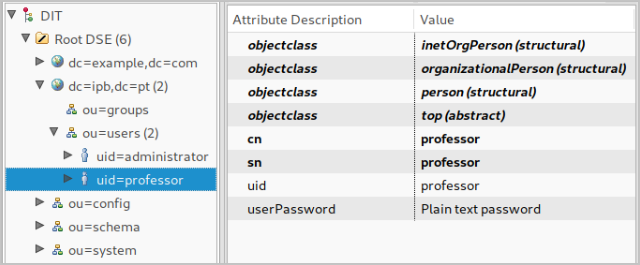
\includegraphics[width=.8\textwidth]{images/screenshots/ldap-directory}
  \caption{Directory structure and the properties of user \texttt{professor}}\label{fig:adsconfig}
\end{figure}

\subsection{Database Initializer}
When starting \gls{Yabi} for the first time, it needs to generate its database, create the root permission and an administrator account.
To do so, the class \texttt{DbInitializer} was written. It implements the \texttt{CommandLineRunner} interface so that Spring instantiate and runs it upon initialization.

There are two properties that interact with \texttt{DbInitializer}, \texttt{yabi.db.init} and \texttt{yabi.db.init.admin.username}. The former regulates when yabi should create a new database, the root permission and the administrator account, the latter declares the administrator's username that should be used. If the initialization is desired, \texttt{yabi.db.init} should be set to \texttt{create}, otherwise, it should be set to anything else. It is necessary that the administrator username is able to be bound in the directory service otherwise the authentication will fail.

\subsection{Postman Tests}
When developing the \gls{API}, some test cases were created in Postman to assess the prevention of data duplication. All four entities were tested.
In essence, every test consists of two requests, one that creates a new entity and expects a \gls{HTTP} status 201 response and the other that tries to re-create the same entity and expects a \gls{HTTP} status 409.

It is important to note that these tests are validating the following restrictions imposed in each entity:
\begin{itemize}
\item There must be only one \texttt{PermissionTree} per \texttt{nodePath}.
\item One \texttt{Directory} per \texttt{connectionString} so that each database is referenced once.
\item One \texttt{Directory} per \texttt{name} so that each name maps to only one database.
\item One \texttt{SqlQuery} under a \texttt{PermissionTree} with a given \texttt{name}, avoiding ambiguous \texttt{SqlQuery} entries.
\item No more than one \texttt{YabiUser} with a given \texttt{name}.
\end{itemize}

\subsection{Conclusion}
This section discussed the implementation details all the parts that compose the \gls{Yabi} application and its development.
\todo{conclusao da implementação}




\cleardoublepage
\chapter{Conclusion}

With the growing adoption of digital processes by companies and institutions, the access to information becomes less available to the general public and more focused to experts in the field. These experts then end up mediating the interaction between those who are part of the decision-making process and the information storage.

Being in this situation, \gls{IPB}'s \gls{IT} department is often interrupted form their daily tasks to handle the most diverse inquiry and questions about the institution's data base.

The present system is designed to aid everyone that takes part in this process as it is able to provide int a efficient and organized manner digital information without the need for much technical knowledge, which in turn lowers the amount of daily interruptions in the \gls{IT} department.
% end of recapitulacao
% capacidades
It currently achieves this by providing a web interface in which the institution members can login, choose one of the many inquiries registered by the \gls{IT} department and download its results, lowering the amount of daily interruptions.

% o que ficou ruim
In the end, some functionalities were not implemented. The most missed one is the ability for the users to tweak their inquiries to similar but specific needs.
% O que ficou bom
In spite of this the final system accomplishes the main task of providing users with the most used inquiries provided that the \gls{IT} department registers them. Not only providing the inquiries, it also supplies the necessary tools to manage users, permissions and remote databases, all through a web interface.
\cleardoublepage
\chapter{Future Work}


\section{Code Re-structure}
\subsection{Administrative Resources}
Currently, resource filtering is implemented by having a small set of controllers that are eligible to handle non-administrative users however this led to some confusion because its response structure does not follow the \gls{HATEOAS} convention.

Some re-structuring could be done at the repository level by configuring the authorization mechanism to filter \gls{HTTP} methods based on the current user's requesting role.

Ultimately, all resources should follow the \gls{HATEOAS} pattern so that the complexity of the front-end application is lower.

\subsection{Bullk information manager}

\todo{}

%% estilo de referências. outros valores posíveis são 'plain' e 'abbrv' apalike
%\bibliographystyle{plain}
%% listagem de referências
%\bibliography{lib/refs}

%  Caso seja usado biblatex
\printbibliography

% Apêndices
\appendix

%http://tex.stackexchange.com/questions/59572/custom-page-numbering-for-appendix
\pretocmd{\chapter}{%
	\clearpage
	\pagenumbering{arabic}%
	\renewcommand*{\thepage}{\thechapter\arabic{page}}%
}{}{}

\chapter{Proposta Original do Projeto}
\label{apendice1}

\begin{figure}
%\centering 
\hspace{-12ex}
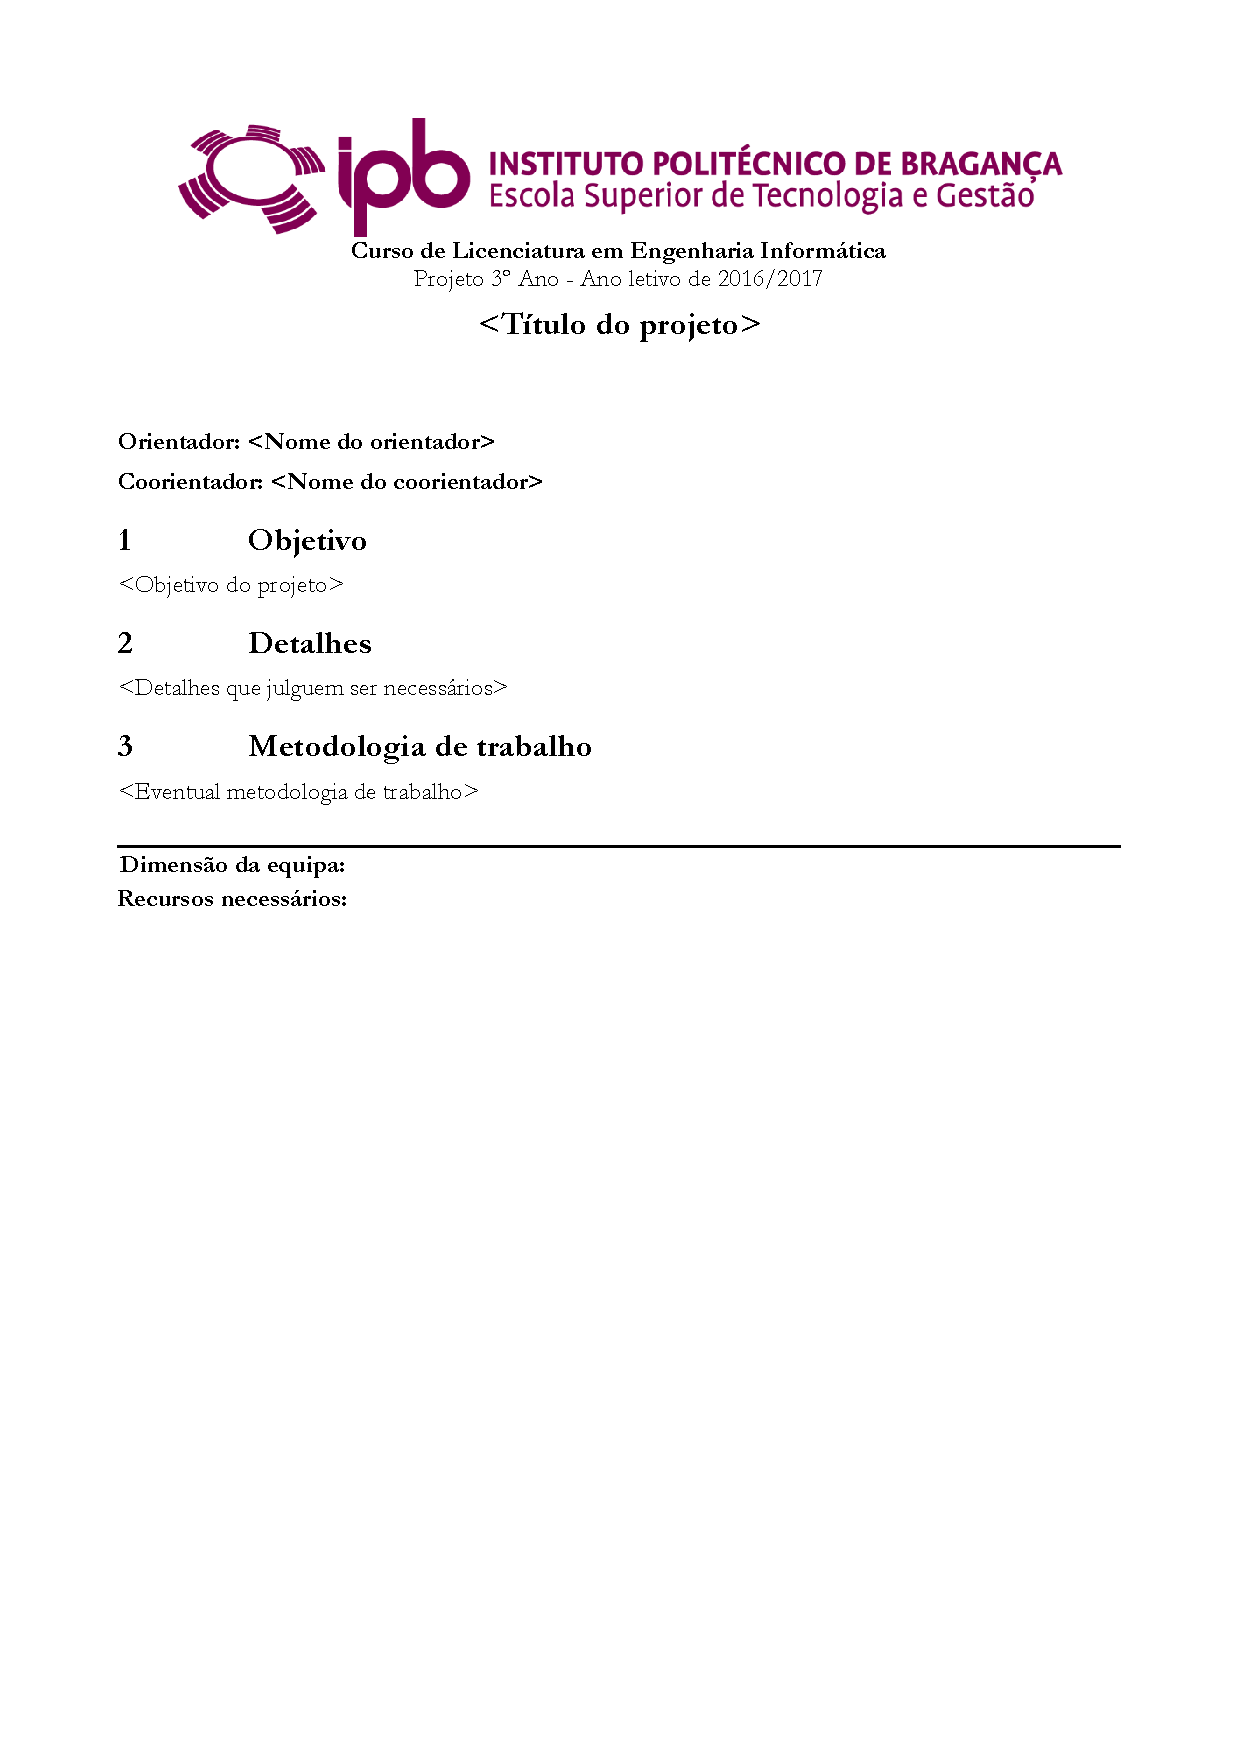
\includegraphics{etc/PropostaProjeto.pdf}
\end{figure}
% \chapter{Outro(s) Apêndice(s)}
\label{apendice2}

Listagens de código fonte, texto/imagens produzidos por testes complementares, etc.


\end{document}
